\documentclass{article}

\title{Metodi Numerici per l'Informatica}
\author{Anthony}
\date{12 apr 2023}

\usepackage{amssymb}
\usepackage{amsmath}
\usepackage{graphicx}

\begin{document}
    \maketitle
    \section{Introduzione}
        \subsection{Isometrie}
            Abbiamo già visto che le matrici ortogonali preservano le lunghezze:
            \[ \Vert \mathbf{Qx} \Vert_2^2 = \mathbf{x}^T\mathbf{Q}^T\mathbf{Qx} = \mathbf{x}^T\mathbf{Ix} = \mathbf{x}^T\mathbf{x} = \Vert \mathbf{x} \Vert_2^2 \]
            E preservano anche gli angoli (prodotti interni):
            \[\langle \mathbf{Qx} , \mathbf{Qy} \rangle = \mathbf{x}^T\mathbf{Q}^T\mathbf{Qy} = \mathbf{x}^T\mathbf{Iy} = \mathbf{x}^T\mathbf{y}\]
            Per queste proprietà, la mappa $\mathbf{x} \mapsto \mathbf{Qx}$ è un'isometria di $\mathbb{R}^n$.
        \subsection{Introduzione a SVD}
            In generale, una trasformazione lineare generale può sempre essere fattorizzata come segue:
            \[ \underbrace{\mathbf{A}}_{m \times n} = \underbrace{\mathbf{U}}_{m \times m} \underbrace{\mathbf{\Sigma}}_{m \times n} \underbrace{\mathbf{V}^T}_{n \times n}\]
            In cui:
            \begin{enumerate}
                \item $\mathbf{U}$ e $\mathbf{V}$ sono matrici ortogonali diverse
                \item $\mathbf{\Sigma}$ è una matrice rettangolare alta o larga, ad esempio: \footnotesize{$\begin{pmatrix}
                    \sigma_1 & 0 & 0 & 0 & 0 \\
                    0 & \sigma_2 & 0 & 0 & 0 \\
                    0 & 0 & \sigma_3 & 0 & 0
                \end{pmatrix}$}
            \end{enumerate}
            Questa decomposizione si chiama \emph{decomposizione a valori singolari (SVD)}.
            \begin{center}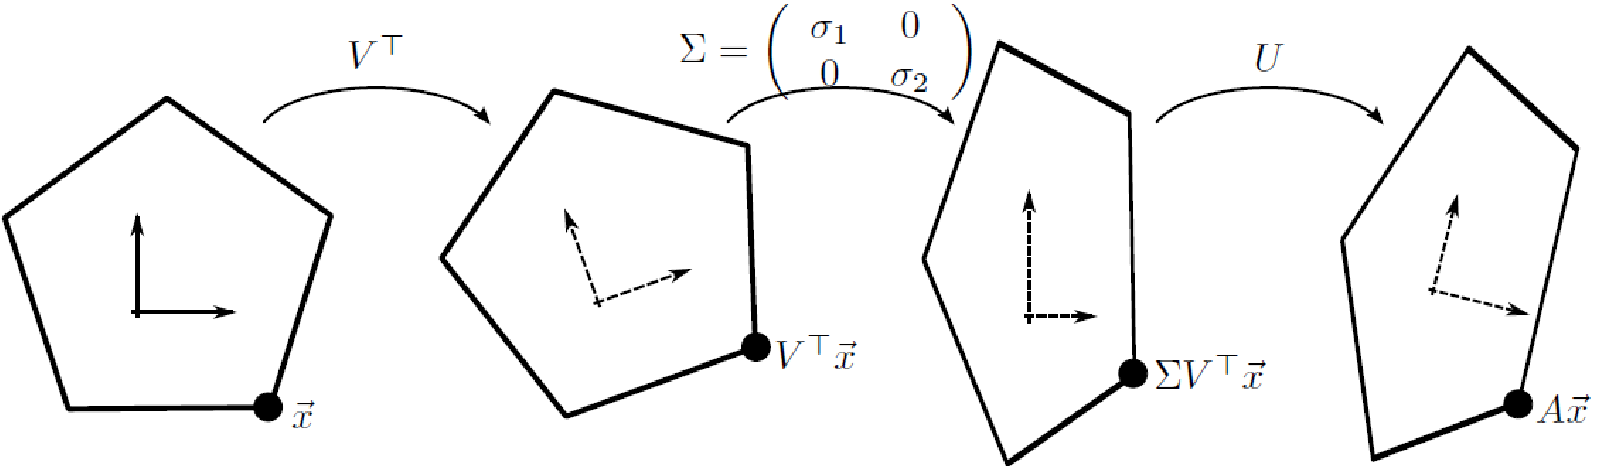
\includegraphics[width=12cm]{singular_val.png}\end{center}
            Tale decomposizione possiamo anche scriverla come segue:
            \[\mathbf{AV} = \mathbf{U\Sigma}\]
            Che somiglia molto all'equazione agli autovalori.
            \paragraph{Serie di prodotti esterni} 
            Possiamo riscrivere la decomposizione $\mathbf{A} = \mathbf{U \Sigma V}^T$ come:
            \[\mathbf{A} = \sum_{i=1}^\ell \sigma_i \mathbf{u}_i\mathbf{v}_i^T\]
            In cui $\mathbf{u}_i$ e $\mathbf{v}_i$ sono le $i$-esime colonne di $\mathbf{U}$ e $\mathbf{V}$ rispettivamente. Possiamo 
            facilmente osservare che ogni prodotto esterno $\mathbf{u}_i\mathbf{v}_i^T$ è una matrice $m \times n$ ed, essendo una matrice 
            rettangolare, possiamo usare semplicemente $\ell = \min{\{m,n\}}$ perché le colonne rimanenti saranno azzerate. \\
            \paragraph{Approssimazione} Se approssimiamo piccoli valori di $\sigma_i$ a zero, stiamo approssimando $\mathbf{A}$ 
            con meno termini:
                \[\mathbf{A} \approx \mathbf{U\tilde{\Sigma}V}^T\]
            in cui $\mathbf{\tilde{\Sigma}}$ è come $\mathbf{\Sigma}$ ma ha i valori $\sigma_i$ piccoli troncati a zero. Possiamo quindi costruire la matrice:
            \[\tilde{\mathbf{A}} \equiv \mathbf{U\tilde{\Sigma}V}^T\]
            troncando ai primi $k$ valori singolari più grandi, azzerando tutti gli altri a zero.
            \subsection{Teorema di Eckart-Young}
            La matrice $\mathbf{A} \approx \mathbf{U\tilde{\Sigma}V}^T$ minimizza l'errore $\Vert \mathbf{A} - \tilde{\mathbf{A}} \Vert_F$ 
            soggetto al vincolo che lo spazio delle colonne di $\mathbf{\tilde{A}}$ ha al più $k$ dimensioni. Questo ci porta 
            a un'approssimazione \emph{low rank} della matrice iniziale $\mathbf{A}$.
\end{document}